%----------------------------------------------------------
\chapter{Архитектура программной реализации}\label{chap3_soft_architecture}
%----------------------------------------------------------
Проектирование новой программной архитектуры графового модуля библиотеки comsdk проводилось с учётом доступа разработчика к средствам стандартной библиотеки языка C++ стандарта C++-11 и библиотеки шаблонных классов Standart Template Library (STL).
\section{Узлы и рёбра графа}
Структура разработанных классов узла графа (\textsf{Node}) и ребра (\textsf{Edge}) представлена на рисунках \ref{fig:classNode}~и~\ref{fig:classEdge} соответственно.
\begin{figure}[!ht]
    \centering
    \begin{minipage}{0.455\textwidth}
        \centering
        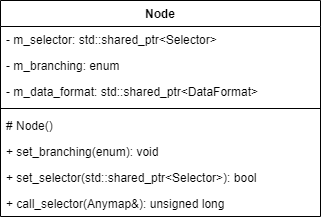
\includegraphics[width=0.9\textwidth]{figures/class.node.png}
        \caption{Класс узла графа}
        \label{fig:classNode}
    \end{minipage}\hfill
    \begin{minipage}{0.455\textwidth}
        \centering
        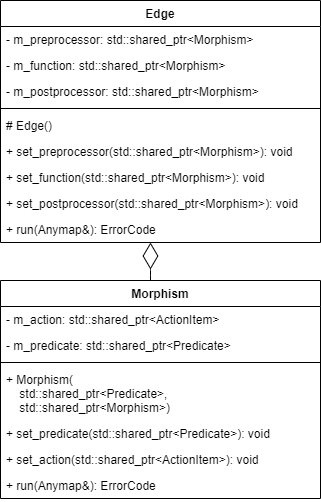
\includegraphics[width=0.9\textwidth]{figures/class.edge.png}
        \caption{Класс ребра графа}
        \label{fig:classEdge}
    \end{minipage}
\end{figure}

Класс узла содержит в себе объект, описывающий состояние данных \textsf{DataFormat}, указатель на объект класса \textsf{Selector} и тип стратегии параллельного выполнения исходящих из него рёбер. Кроме того класс \textsf{Node} предоставляет интерфейс для назначения и вызова селектора и назначения стратегии распараллеливания. В свою очередь класс \textsf{Selector} является обёрткой над функтором, который по входным данным создаёт массив логических переменных, где 1 на \(i\)-той позиции означает, что при обходе необходимо выполнить \(i\)-тое ребро, выходящее из узла. Класс ребра предоставляет интефейс для назначения ему до трёх морфизмов и их выполнения, что в полной мере соответствует обозначенным в разделе~\ref{section:requirements} требованиям.

\section{Хранение узлов и рёбер графа}
Задача хранения данных узлов и рёбер была отведена непосредственно классу графа (\textsf{Graph}). Поскольку основной операцией с узлами и рёбрами является обращение к ним по их индексу, в качестве контейнеров для них были выбраны динамиические массивы (\textsf{std::vector}). Кроме того, данному классу была отведена задача хранить данные о топологии графовой модели в виде матрицы смежности. Данное решение позволяет легко проверять наличие ребра между двумя узлами и, кроме того, даёт возможность сразу узнать индекс ребра при его существовании. Поскольку граф должен формироваться засчёт поочерёдного добавления в него узлов и рёбер, в качестве контейнера для этой матрицы был взят двумерный динамический массив. UML-диаграмма данного класса приведена на рисунке~\ref{fig:classGraph}.
\begin{figure}[!ht]
    \centering
    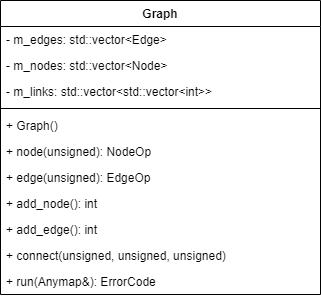
\includegraphics[height=6cm]{figures/class.graph.png}
    \caption{Класс графа}
    \label{fig:classGraph}
\end{figure}

Помимо этого для удобства доступа к структуре графа во время обхода были спроектированы две вспомогательные структуры данных, позволяющих отделить данные о топологии графа от отдельно взятых узлов и рёбер. UML-диаграммы этих структур представлены на рисунке~\ref{fig:additionalGraphStructure}.
\begin{figure}[!ht]
    \centering
    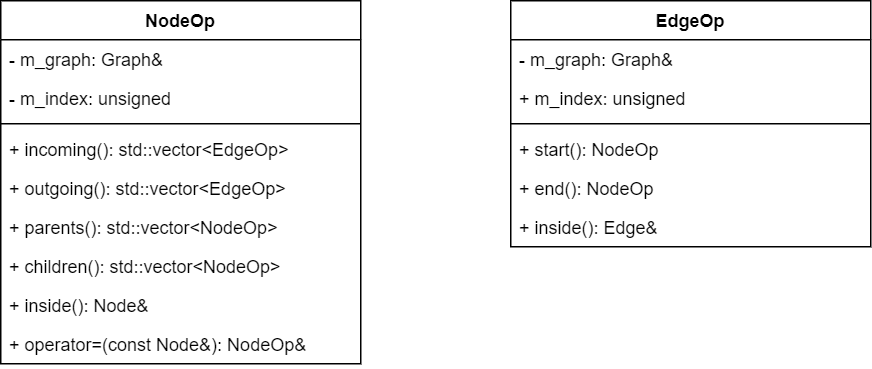
\includegraphics[height=5cm]{figures/structure_additional.png}
    \caption{Дополнительные структуры данных}
    \label{fig:additionalGraphStructure}
\end{figure}

Например, класс \textsf{NodeOp} предоставляет интерфейс для получения входящих и выходящих рёбер для конкретного узла, соседних узлов и при необходимости позволяет обратиться непосредственно к интерфейсу самого узла, при этом внутри объекта этого класса хранится только ссылка на граф и индекс узла, что позволяет эффективно использовать память, когда необходимости обращаться к интерфейсу самого узла нет. Аналогично в классе \textsf{EdgeOp} хранится только индекс ребра и ссылка на граф. Интерфейс данного класса позволяет получить начальную и конечную вершины для данного ребра и при необходимости обратиться к интерфейсу самого ребра (\textsf{Edge}).

Итоговая UML-диаграмма классов, спроектированных в рамках графового модуля comsdk представлена на рисунке~\ref{fig:suggestedGraphStructure}.
\begin{figure}[!ht]
    \centering
    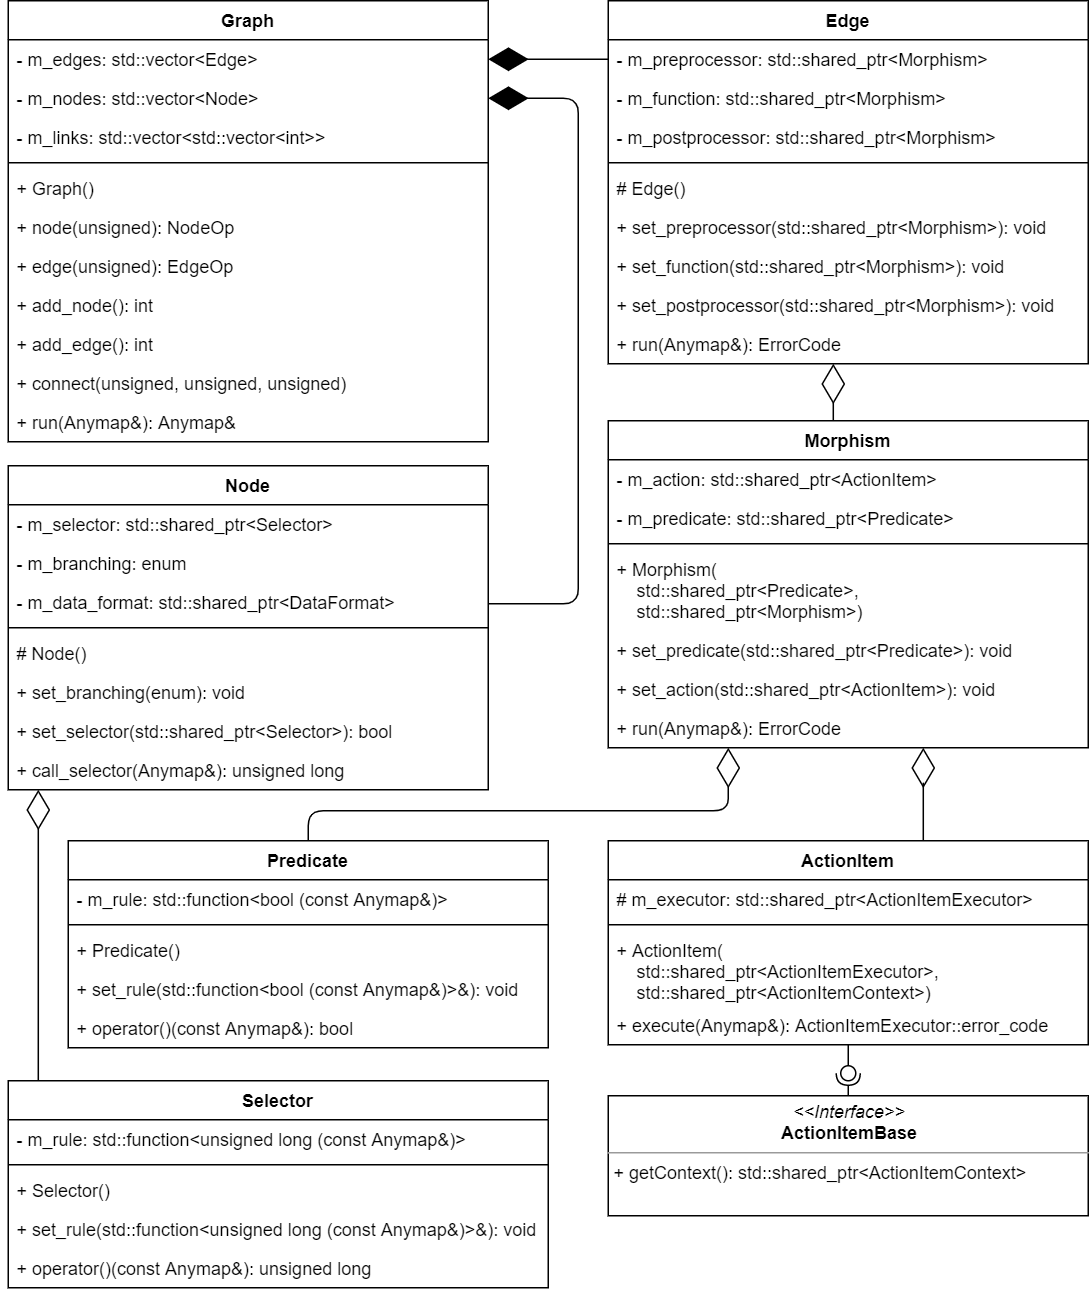
\includegraphics[width=\textwidth]{figures/suggested_structure.png}
    \caption{Предлагаемая структура классов}
    \label{fig:suggestedGraphStructure}
\end{figure}
%----------------------------------------------------------
%\section{...}

%----------------------------------------------------------

